\section{Introduction}

The goal of the project is to computationally determine the similarity of the
16 selected Philippine Languages which are enumerated
in~\cref{tab:ph_languages}. The GitHub repository of the project may be
accessed here:
\begin{center}
    \url{https://github.com/zrygan/nlp}
\end{center}

The Philippines is an archipelago of more than 7,600
islands in three groups: Luzon in the north, the Visayas in the centre, and
Mindanao in the south. Its mountainous terrain and the sea channels dividing its
islands have historically both restricted and channelled contact between
language communities~\cite{Boquet_2017}.

Tagalog, Kapampangan, and Pangasinan are spoken across the plains of Central
Luzon; further north, Ilocano occupies the coastal lowlands, Adasen the
Cordillera interior of Abra, and Paranan the Sierra Madre coast facing the
Pacific. The Visayas hold a contiguous but diversified cluster of Bisayan
languages, namely Cebuano, Hiligaynon, Kinaray-a, and Waray-Waray, divided by
narrow sea channels, with Bikol, Masbatenyo, and Romblomanon in the transitional
zone between the Visayas and Luzon. In the south, Tausug is spoken in the Sulu
archipelago and Chavacano, a Spanish-based creole, in Zamboanga. Yami alone lies
outside the Philippines, on Orchid Island off southeastern Taiwan; a Batanic
language closest to the Ivatan of Batanes, it is included as a northern
Austronesian outgroup. Below in \cref{fig:lingmap_out} shows the image of
what the linguistic map looks like.

\begin{figure}[h]
    \centering
    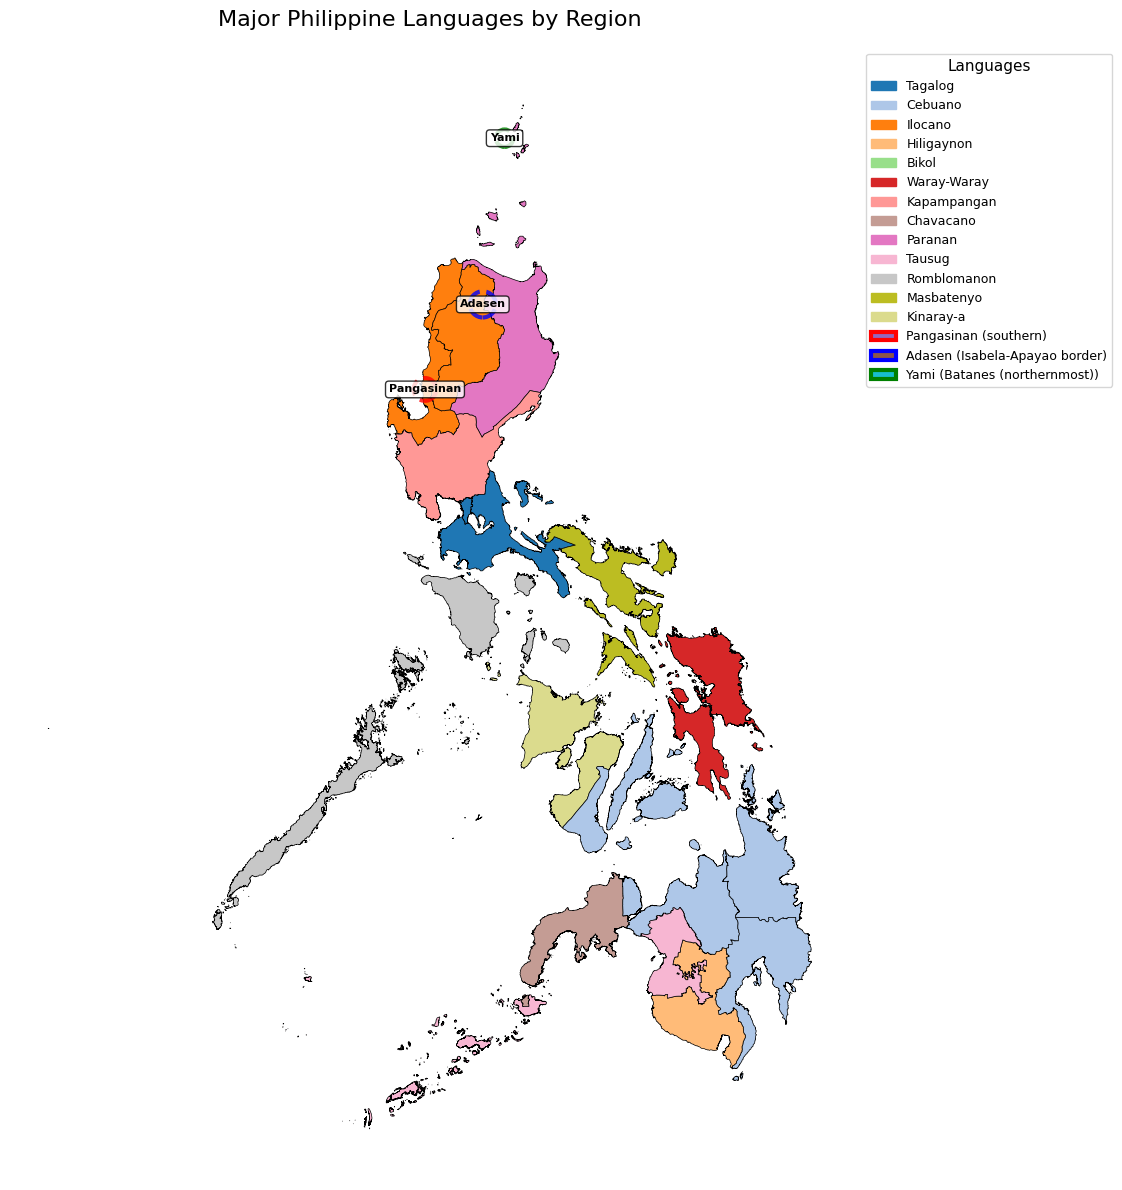
\includegraphics[width=\columnwidth]{chapters/artifacts/lingmap_out.png}
    \caption{Generated linguistic map showing the spatial distribution of the
        selected Philippine languages overlaid on topographic contours. Its
        construction is described in~\cref{sec:geo}.}
    \label{fig:lingmap_out}
\end{figure}

The corpora used for the orthographic and phonetic similarity were collected by
the authors from Biblical translations, and are not drawn from any published
dataset. The collection procedure is documented in full
in~\cref{sec:data_collection} rather than by reference to an external source,
and the ethical and contractual questions it raises are stated
in the~\nameref{sec:ethics_stmt} and analysed in~\cref{sec:ethics}.